\documentclass{article}

\usepackage{hyperref}
\hypersetup{
	colorlinks=true,
	linkcolor=blue,
	urlcolor=cyan,}
\usepackage{booktabs}
\usepackage{textgreek}

%%%%%%%%%%%%%%%%%%%%%%%%%%%%%%%%%%%%%%%%%
% Lachaise Assignment
% Structure Specification File
% Version 1.0 (26/6/2018)
%
% This template originates from:
% http://www.LaTeXTemplates.com
%
% Authors:
% Marion Lachaise & François Févotte
% Vel (vel@LaTeXTemplates.com)
%
% License:
% CC BY-NC-SA 3.0 (http://creativecommons.org/licenses/by-nc-sa/3.0/)
% 
%%%%%%%%%%%%%%%%%%%%%%%%%%%%%%%%%%%%%%%%%

%----------------------------------------------------------------------------------------
%	PACKAGES AND OTHER DOCUMENT CONFIGURATIONS
%----------------------------------------------------------------------------------------

\usepackage{amsmath,amsfonts,stmaryrd,amssymb} % Math packages

\usepackage{enumerate} % Custom item numbers for enumerations

\usepackage[ruled]{algorithm2e} % Algorithms

\usepackage[framemethod=tikz]{mdframed} % Allows defining custom boxed/framed environments

\usepackage{listings} % File listings, with syntax highlighting
\lstset{
	basicstyle=\ttfamily, % Typeset listings in monospace font
}

%----------------------------------------------------------------------------------------
%	DOCUMENT MARGINS
%----------------------------------------------------------------------------------------

\usepackage{geometry} % Required for adjusting page dimensions and margins

\geometry{
	paper=a4paper, % Paper size, change to letterpaper for US letter size
	top=2.5cm, % Top margin
	bottom=3cm, % Bottom margin
	left=2.5cm, % Left margin
	right=2.5cm, % Right margin
	headheight=14pt, % Header height
	footskip=1.5cm, % Space from the bottom margin to the baseline of the footer
	headsep=1.2cm, % Space from the top margin to the baseline of the header
	%showframe, % Uncomment to show how the type block is set on the page
}

%----------------------------------------------------------------------------------------
%	FONTS
%----------------------------------------------------------------------------------------

\usepackage[utf8]{inputenc} % Required for inputting international characters
\usepackage[T1]{fontenc} % Output font encoding for international characters

\usepackage{XCharter} % Use the XCharter fonts

%----------------------------------------------------------------------------------------
%	COMMAND LINE ENVIRONMENT
%----------------------------------------------------------------------------------------

% Usage:
% \begin{commandline}
%	\begin{verbatim}
%		$ ls
%		
%		Applications	Desktop	...
%	\end{verbatim}
% \end{commandline}

\mdfdefinestyle{commandline}{
	leftmargin=10pt,
	rightmargin=10pt,
	innerleftmargin=15pt,
	middlelinecolor=black!50!white,
	middlelinewidth=2pt,
	frametitlerule=false,
	backgroundcolor=black!5!white,
	frametitle={Command Line},
	frametitlefont={\normalfont\sffamily\color{white}\hspace{-1em}},
	frametitlebackgroundcolor=black!50!white,
	nobreak,
}

% Define a custom environment for command-line snapshots
\newenvironment{commandline}{
	\medskip
	\begin{mdframed}[style=commandline]
}{
	\end{mdframed}
	\medskip
}

%----------------------------------------------------------------------------------------
%	FILE CONTENTS ENVIRONMENT
%----------------------------------------------------------------------------------------

% Usage:
% \begin{file}[optional filename, defaults to "File"]
%	File contents, for example, with a listings environment
% \end{file}

\mdfdefinestyle{file}{
	innertopmargin=1.6\baselineskip,
	innerbottommargin=0.8\baselineskip,
	topline=false, bottomline=false,
	leftline=false, rightline=false,
	leftmargin=2cm,
	rightmargin=2cm,
	singleextra={%
		\draw[fill=black!10!white](P)++(0,-1.2em)rectangle(P-|O);
		\node[anchor=north west]
		at(P-|O){\ttfamily\mdfilename};
		%
		\def\l{3em}
		\draw(O-|P)++(-\l,0)--++(\l,\l)--(P)--(P-|O)--(O)--cycle;
		\draw(O-|P)++(-\l,0)--++(0,\l)--++(\l,0);
	},
	nobreak,
}

% Define a custom environment for file contents
\newenvironment{file}[1][File]{ % Set the default filename to "File"
	\medskip
	\newcommand{\mdfilename}{#1}
	\begin{mdframed}[style=file]
}{
	\end{mdframed}
	\medskip
}

%----------------------------------------------------------------------------------------
%	NUMBERED QUESTIONS ENVIRONMENT
%----------------------------------------------------------------------------------------

% Usage:
% \begin{question}[optional title]
%	Question contents
% \end{question}

\mdfdefinestyle{question}{
	innertopmargin=1.2\baselineskip,
	innerbottommargin=0.8\baselineskip,
	roundcorner=5pt,
	nobreak,
	singleextra={%
		\draw(P-|O)node[xshift=1em,anchor=west,fill=white,draw,rounded corners=5pt]{%
		Question \theQuestion\questionTitle};
	},
}

\newcounter{Question} % Stores the current question number that gets iterated with each new question

% Define a custom environment for numbered questions
\newenvironment{question}[1][\unskip]{
	\bigskip
	\stepcounter{Question}
	\newcommand{\questionTitle}{~#1}
	\begin{mdframed}[style=question]
}{
	\end{mdframed}
	\medskip
}

%----------------------------------------------------------------------------------------
%	WARNING TEXT ENVIRONMENT
%----------------------------------------------------------------------------------------

% Usage:
% \begin{warn}[optional title, defaults to "Warning:"]
%	Contents
% \end{warn}

\mdfdefinestyle{warning}{
	topline=false, bottomline=false,
	leftline=false, rightline=false,
	nobreak,
	singleextra={%
		\draw(P-|O)++(-0.5em,0)node(tmp1){};
		\draw(P-|O)++(0.5em,0)node(tmp2){};
		\fill[black,rotate around={45:(P-|O)}](tmp1)rectangle(tmp2);
		\node at(P-|O){\color{white}\scriptsize\bf !};
		\draw[very thick](P-|O)++(0,-1em)--(O);%--(O-|P);
	}
}

% Define a custom environment for warning text
\newenvironment{warn}[1][Warning:]{ % Set the default warning to "Warning:"
	\medskip
	\begin{mdframed}[style=warning]
		\noindent{\textbf{#1}}
}{
	\end{mdframed}
}

%----------------------------------------------------------------------------------------
%	INFORMATION ENVIRONMENT
%----------------------------------------------------------------------------------------

% Usage:
% \begin{info}[optional title, defaults to "Info:"]
% 	contents
% 	\end{info}

\mdfdefinestyle{info}{%
	topline=false, bottomline=false,
	leftline=false, rightline=false,
	nobreak,
	singleextra={%
		\fill[black](P-|O)circle[radius=0.4em];
		\node at(P-|O){\color{white}\scriptsize\bf i};
		\draw[very thick](P-|O)++(0,-0.8em)--(O);%--(O-|P);
	}
}

% Define a custom environment for information
\newenvironment{info}[1][Info:]{ % Set the default title to "Info:"
	\medskip
	\begin{mdframed}[style=info]
		\noindent{\textbf{#1}}
}{
	\end{mdframed}
}
 % Include the file specifying the document structure and custom commands

%----------------------------------------------------------------------------------------
%	ASSIGNMENT INFORMATION
%----------------------------------------------------------------------------------------

\title{EMG Lab 3: EMG Circuit}
\author{BIOE 385 Bioinstrumentation Laboratory} 
\date{}
%----------------------------------------------------------------------------------------

\begin{document}
\large
\maketitle

\section*{Goals}
\begin{enumerate}
	\item Determine the amplitude and frequency range of an EMG signal
	\item Explain how the electrical isolation circuit built in class works to protect the patient from the risk of exposure to high voltages or currents in the event of component failure
	\item Design a circuit to amplify and filter an EMG signal
	\item Justify the selection of components used to amplify the EMG signal (ie. 2-stage amplification, gain, instrumentation amplifiers, etc)
	\item Use OP07 and AD620 instrumentation amplifiers to design circuits.  
\end{enumerate}

\section*{Pre-lab Assignment}
Describe two possible sites in which you could place electrodes to measure a reflex response using your hammer. Determine and write down the size and frequency range of the EMG signal you would like to collect. If you are told to make a band pass filter, what frequencies will be your cut off frequencies? Design and draw out this band-pass filter. How might you handle potential 60Hz noise in your signal?

\section*{In-lab Assignment}
\subsection*{Safety and Electrical Isolation}

\begin{figure}[h]
    	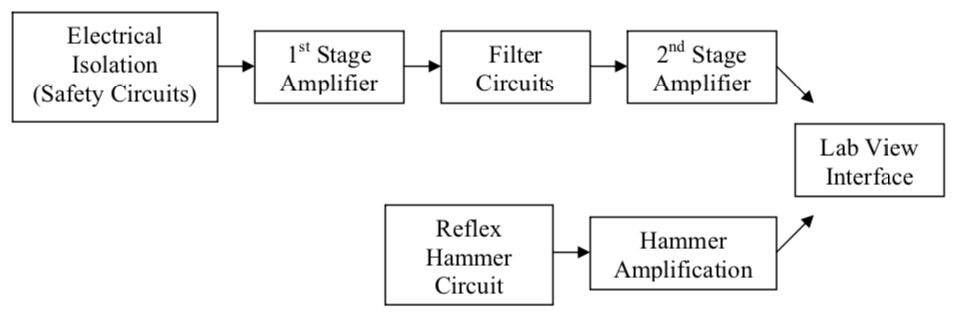
\includegraphics[width=0.9\textwidth]{lab_3_fig_1.jpg}
    	\centering
		\end{figure}	

\begin{warn}
It is critical that you follow this next set of instructions EXACTLY.	
\end{warn}

In order to protect the patient from the risk of exposure to high voltages or current in the event of component failure, we will add an electrical isolation circuit between the patient and the measurement instrument. When the voltage across the diode exceeds around +0.6 V, current can flow in one direction only. Add the following circuit to each input of the instrumentation amplifier (not necessary for the ground electrode.)\\

\begin{figure}[h]
    	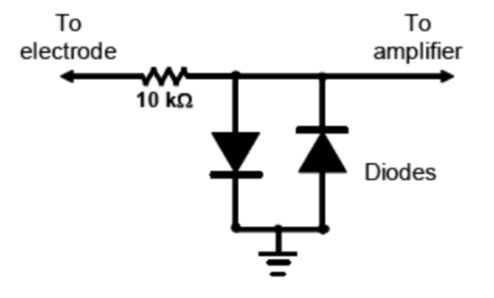
\includegraphics[width=0.4\textwidth]{lab_3_fig_2.jpg}
    	\centering
		\end{figure}	

If the voltage at the amplifier input exceeds 0.6 V, then the diodes will provide a low impedance route for the current to flow to ground, rather than the patient. Hint: The input connections to the amplifier are the most susceptible points for picking up noise, so cut the leads short on the diodes, resistors and wires so that they do not form loops sticking up out of the protoboard.\\

After these connections are made, your instructor or TA must check them before you connect any electrodes to the test subject.

\subsection*{EMG Amplification}
Select the GAIN you would like for the EMG signal. You will likely want to amplify the signal in two stages. You will be using an AD620 Instrumentation amplifier (a differential amplifier) for the first amplification stage. Check the SPEC sheet to determine the pin diagram for the AD620. Determine the desired gain in your circuit and calculate the resistors you will need to accomplish this.

\begin{enumerate}
	\item Draw out the circuit you want to build. Specify desired gain and values of components.
	\item Now build the circuit. Test it out using the function generator in ELVIS to be sure it is behaving as you expect. Have your instructor or TA check your circuit prior to trying it out on a test subject.
\end{enumerate}

You may now test and see if you are able to detect your own EMG signal. Notice what happens when the test subject moves their arm around slowly while data are being collected. How can this drift in the signal be filtered out?

\subsection*{Signal Filtering}
Draw and build the filter you would like to have for your device. This part is completely up to you. Do you want active or passive filters? Do you want single stage or higher order filters? The signal coming out of your AD620 OpAmp will need to be filtered. For now, do not worry about 60Hz noise. The 60Hz signal is pervasive and comes from the lights and monitors. To reduce this noise you should move the test subject as far away from the computer as possible for now.\\

After you have filtered the signal, it is likely that you will have attenuated the gain some and you may want to insert a final stage amplification.

\subsection*{Final Amplification}
To get the signal into the value range that you want, you should amplify it one more time. Select the appropriate resistors to get your desired gain. You should use an OP07 Op Amp for this gain.

\end{document}
